\begin{figure}[t]
\centering\footnotesize
\resizebox{\columnwidth}{!}{%
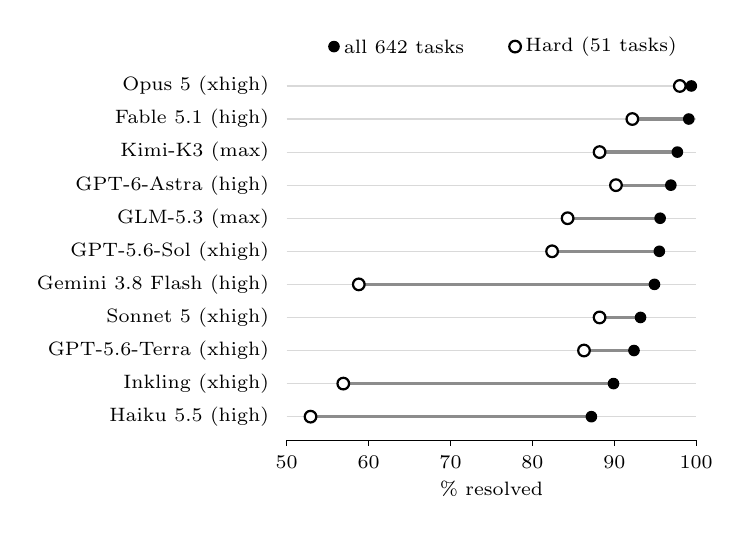
\begin{tikzpicture}
\node[anchor=east,font=\scriptsize] at (-0.1,0.00) {Opus 5 (xhigh)};
\draw[gray!30] (0,0.00) -- (5.2,0.00);
\draw[line width=1.2pt,black!45] (4.992,0.00) -- (5.138,0.00);
\fill[black] (5.138,0.00) circle (2.1pt);
\draw[black,fill=white,line width=0.8pt] (4.992,0.00) circle (2.1pt);
\node[anchor=east,font=\scriptsize] at (-0.1,-0.42) {Fable 5.1 (high)};
\draw[gray!30] (0,-0.42) -- (5.2,-0.42);
\draw[line width=1.2pt,black!45] (4.389,-0.42) -- (5.106,-0.42);
\fill[black] (5.106,-0.42) circle (2.1pt);
\draw[black,fill=white,line width=0.8pt] (4.389,-0.42) circle (2.1pt);
\node[anchor=east,font=\scriptsize] at (-0.1,-0.84) {Kimi-K3 (max)};
\draw[gray!30] (0,-0.84) -- (5.2,-0.84);
\draw[line width=1.2pt,black!45] (3.973,-0.84) -- (4.961,-0.84);
\fill[black] (4.961,-0.84) circle (2.1pt);
\draw[black,fill=white,line width=0.8pt] (3.973,-0.84) circle (2.1pt);
\node[anchor=east,font=\scriptsize] at (-0.1,-1.26) {GPT-6-Astra (high)};
\draw[gray!30] (0,-1.26) -- (5.2,-1.26);
\draw[line width=1.2pt,black!45] (4.181,-1.26) -- (4.878,-1.26);
\fill[black] (4.878,-1.26) circle (2.1pt);
\draw[black,fill=white,line width=0.8pt] (4.181,-1.26) circle (2.1pt);
\node[anchor=east,font=\scriptsize] at (-0.1,-1.68) {GLM-5.3 (max)};
\draw[gray!30] (0,-1.68) -- (5.2,-1.68);
\draw[line width=1.2pt,black!45] (3.567,-1.68) -- (4.742,-1.68);
\fill[black] (4.742,-1.68) circle (2.1pt);
\draw[black,fill=white,line width=0.8pt] (3.567,-1.68) circle (2.1pt);
\node[anchor=east,font=\scriptsize] at (-0.1,-2.10) {GPT-5.6-Sol (xhigh)};
\draw[gray!30] (0,-2.10) -- (5.2,-2.10);
\draw[line width=1.2pt,black!45] (3.370,-2.10) -- (4.732,-2.10);
\fill[black] (4.732,-2.10) circle (2.1pt);
\draw[black,fill=white,line width=0.8pt] (3.370,-2.10) circle (2.1pt);
\node[anchor=east,font=\scriptsize] at (-0.1,-2.52) {Gemini 3.8 Flash (high)};
\draw[gray!30] (0,-2.52) -- (5.2,-2.52);
\draw[line width=1.2pt,black!45] (0.915,-2.52) -- (4.670,-2.52);
\fill[black] (4.670,-2.52) circle (2.1pt);
\draw[black,fill=white,line width=0.8pt] (0.915,-2.52) circle (2.1pt);
\node[anchor=east,font=\scriptsize] at (-0.1,-2.94) {Sonnet 5 (xhigh)};
\draw[gray!30] (0,-2.94) -- (5.2,-2.94);
\draw[line width=1.2pt,black!45] (3.973,-2.94) -- (4.493,-2.94);
\fill[black] (4.493,-2.94) circle (2.1pt);
\draw[black,fill=white,line width=0.8pt] (3.973,-2.94) circle (2.1pt);
\node[anchor=east,font=\scriptsize] at (-0.1,-3.36) {GPT-5.6-Terra (xhigh)};
\draw[gray!30] (0,-3.36) -- (5.2,-3.36);
\draw[line width=1.2pt,black!45] (3.775,-3.36) -- (4.410,-3.36);
\fill[black] (4.410,-3.36) circle (2.1pt);
\draw[black,fill=white,line width=0.8pt] (3.775,-3.36) circle (2.1pt);
\node[anchor=east,font=\scriptsize] at (-0.1,-3.78) {Inkling (xhigh)};
\draw[gray!30] (0,-3.78) -- (5.2,-3.78);
\draw[line width=1.2pt,black!45] (0.718,-3.78) -- (4.150,-3.78);
\fill[black] (4.150,-3.78) circle (2.1pt);
\draw[black,fill=white,line width=0.8pt] (0.718,-3.78) circle (2.1pt);
\node[anchor=east,font=\scriptsize] at (-0.1,-4.20) {Haiku 5.5 (high)};
\draw[gray!30] (0,-4.20) -- (5.2,-4.20);
\draw[line width=1.2pt,black!45] (0.302,-4.20) -- (3.869,-4.20);
\fill[black] (3.869,-4.20) circle (2.1pt);
\draw[black,fill=white,line width=0.8pt] (0.302,-4.20) circle (2.1pt);
\draw (0,-4.50) -- (5.2,-4.50);
\draw (0.000,-4.50) -- (0.000,-4.57) node[below,font=\scriptsize] {50};
\draw (1.040,-4.50) -- (1.040,-4.57) node[below,font=\scriptsize] {60};
\draw (2.080,-4.50) -- (2.080,-4.57) node[below,font=\scriptsize] {70};
\draw (3.120,-4.50) -- (3.120,-4.57) node[below,font=\scriptsize] {80};
\draw (4.160,-4.50) -- (4.160,-4.57) node[below,font=\scriptsize] {90};
\draw (5.200,-4.50) -- (5.200,-4.57) node[below,font=\scriptsize] {100};
\node[font=\scriptsize] at (2.60,-5.12) {\% resolved};
\fill[black] (0.6,0.5) circle (2.1pt) node[right,font=\scriptsize] {all 642 tasks};
\draw[black,fill=white,line width=0.8pt] (2.9,0.5) circle (2.1pt) node[right,font=\scriptsize] {Hard (51 tasks)};
\end{tikzpicture}}
\caption{Percent of tasks resolved on SWE-Bench Pro V2 (filled dots) and its Hard split (open dots). The full set separates these systems by about 12 points (87.2--99.4\%) while the Hard split spans from 52.9\% to 98.0\%.}
\label{fig:spread}
\end{figure}